\chapter{System Analysis}


\requirement{mgmt:create:pipeline}{1110}{Define a new Pipeline}{
	The user must be able to create a new pipeline definition.
	Only valid definitions must be accepted.
	A valid pipeline definition has a name and must contain at least one stage definition.
}
\requirement{mgmt:update:pipeline}{1120}{Update an existing Pipeline}{
	The user must be able to see and modify an existing pipeline definition.
}
\requirement{mgmt:delete:pipeline}{1130}{Delete an existing Pipeline}{
	The user must be able to remove an existing pipeline definition.
	Deleting a pipeline definition must not break and therefore must not prevent associated projects from further execution.
}
\requirement{mgmt:list:pipeline}{1140}{List all Pipelines}{
	The user must be able to retrieve a named list of all existing pipeline definitions.
}

\requirement{mgmt:create:project}{1210}{Create a new Project}{
	The user must be able to create a new project.
	Only valid projects must be accepted.
	A valid project has a name and must be using an existing pipeline definition.
}
\requirement{mgmt:update:project:pipeline}{1220}{Update the Pipeline of a Project}{
	The user must be able to change the pipeline definition an existing project is based on.
}
\requirement{mgmt:update:project:name}{1230}{Update the Name of a Project}{
	The user must be able to update the name of a project.
}
\requirement{mgmt:update:project:labels}{1240}{Updating Tags of a Project}{
	The user must be able to add and remove tags to and from an existing project.
}
\requirement{mgmt:delete:project}{1250}{Delete an existing Project}{
	The user must be able to delete a Project.
	Deleting a project must delete all associated files, directories and configuration files.
}
\requirement{mgmt:list:project}{1260}{List all Projects}{
	The user must be able to retrieved a named list of all existing projects.
}

\requirement{files:upload}{1310}{Upload Files}{
	The user must be able to upload files into the scope of a project, so that further stage execution is able to retrieve said file.
}
\requirement{files:download}{1320}{Download Files}{
	The user must be able to download files that are within the scope of a project.
	Said files can be files that were previously uploaded by the user or are results of executed stages.
}
\requirement{files:list}{1340}{List Files}{
	The user must be able to retrieve a list of files associated with a project.
}

\requirement{exec:start:stage}{1410}{Start a Stage}{
	The user must be able to start a new Stage for a project.
	Any Stage defined in the associated Pipeline Definition is considered a valid choice.
	The user shall be able to choose whether the following Stages shall be executed automatically or the pipeline shall be paused upon completion.
}
\requirement{exec:pause:stage}{1420}{Pause a Pipeline}{
	The user must be able to mark a running Pipeline of a Project to be paused before executing the next Stage.
}
\requirement{exec:resume:stage}{1430}{Resume a Pipeline}{
	The user must be able to resume paused Pipelines.
}
\requirement{exec:abort:stage}{1440}{Abort a running Stage}{
	The user must be able to commit an abort request for a running Stage.
	An aborted Stage shall be considered failed and further Stage execution shall be paused.
}
\requirement{exec:inspect:logs}{1450}{Inspect logs of a Stage}{
	The user must be able to see log messages produced by a selected Stage as well as to that stage associated system events.
}
\requirement{exec:inspect:state}{1460}{Inspect state a Stage}{
	The user must be able to retrieve the state ('RUNNING', 'PAUSED', 'SUCCEEDED', 'FAILED') for all stages of a project.
}

\requirement{node:monitor:cpu}{1510}{Monitor CPU usage}{
	The user must be able to retrieve the CPU utilization of all known nodes.
}
\requirement{node:monitor:ram}{1520}{Monitor RAM usage}{
	The user must be able to retrieve the RAM utilization of all known nodes.
}
\requirement{node:monitor:netio}{1520}{Monitor Network IO}{
	The user must be able to retrieve the Network IO utilization of all known nodes.
}


This chapter is about analysing the to be implemented system.
It is important to find an architecture that is able to fulfil all requirements and that is able to be evolved for upcoming needs.
But, as the YAGNI (\enquote{You Ain't Gonna Need It} \cite[36]{goll2018entwurfsprinzipien}) principle describes, this does not mean one should plan for speculative events.
In some areas where changes or extensions are foreseeable, preparations can be considered, whereas if there is no such indication, one should only consider the actual and current need.
In addition, keeping the SOLID\footnote{\enquote{\textbf{S}ingle-responsibility principle}, \enquote{\textbf{O}open-close principle}, \enquote{\textbf{L}iskov-substitution principle}, \enquote{\textbf{I}nterface segregation principle} and \enquote{\textbf{D}ependency-inversion principle}}\cite[86]{martin2003agile} principles in mind can help to improve correctness, simplicity, stability, changeability and testability\cite[162]{goll2018entwurfsprinzipien}.


The analysis and design in this thesis follows the \enquote{Top-Down} approach\cite[171]{goll2012methoden} in which the system is first generally outlined and then step by step partitioned into smaller and more detailed pieces.


%\todo{mention? decentralization aspects?}

\pagebreak
\section{System Context}
%\todo{.delete?}

A System Context Diagram is suitable to find the boundaries of the system to implement and interactions with external components.
The first step was therefore to create \autoref{system_context_diagramm}.
The notation is a slight deviation from the UML standard so that the control and data flow can also be displayed \cite[501]{goll2012methoden}.

\begin{figure}[H]
	\begin{tikzpicture}[node distance=5,scale=0.8, every node/.style={transform shape}]
		\node [draw, rectangle, drop shadow, fill=white] (F) {User};
		\node [draw, circle, drop shadow, fill=white, text width=3cm, align=center] (C) [below right=of F] {Winslow};
		\node [draw, rectangle, drop shadow, fill=white] (S) [below right=of C] {Storage};
		\node [draw, rectangle, drop shadow, fill=white] (A) [above right=of C] {Stage Execution};
		
		\node (ctrl1) [above=of S] {};
		\node (ctrl2) [above right=of C] {};
		\node (ctrl3) [right=of C] {};
		\node (ctrl4) [below=of F] {};
		\node (ctrl5) [left=of C] {};
		\node (ctrl6) [below=of ctrl5] {};
		\node (ctrl7) [above=of C] {};
		\node (ctrl8) [right=of F] {};
		\node (ctrl9) [below left=of C] {};
		\node (ctrl10) [below=of C] {};
		
		%
		% User -> Winslow
		%
		\path[draw, -{Latex[scale=2.0]}, dashed] (F)
			edge [bend right] node [fill=white] {manage project} (C)
			edge [bend left]  node [fill=white] {manage execution} (C)
			.. controls (ctrl7) and (ctrl8) ..  node [fill=white] {monitor} (C);
			
		\path[draw, -{Latex[scale=2.0]}] (F)
			edge node [fill=white] {input video} (C);
		
		%
		% Winslow -> User
		%
		\path[draw, -{Latex[scale=2.0]}] (C)
			.. controls (ctrl4) and (ctrl5) ..  node [fill=white] {results} (F);
		
		%
		% Winslow -> Stage Execution
		%
		\path[draw, -{Latex[scale=2.0]}, dashed] (C)
			edge [bend left] node [fill=white] {create} (A)
			edge [bend right] node [fill=white] {destroy} (A);
			
		%
		% Stage Execution -> Winslow
		%
		\path[draw, -{Latex[scale=2.0]}] (A)
			edge node [fill=white] {logs \& satus} (C);
		
		%
		% Storage -> Winslow
		%		
%		\path[draw, -{Latex[scale=2.0]}] (S)
%			edge node [fill=white] {configuration} (C)
%			.. controls (ctrl3) and (ctrl1) ..  node [fill=white] {resource files} (C);
		
		%
		% Winslow -> Storage
		%
		\path[draw, {Latex[scale=2.0]}-{Latex[scale=2.0]}] (C)
			edge [bend left]  node [fill=white] {configuration} (S)
			edge [bend right] node [fill=white] {input files} (S)
			edge node [fill=white] {results} (S);
		
		
		\path[draw, {Latex[scale=2.0]}-{Latex[scale=2.0]}, dashed] (C)
			.. controls (ctrl10) and (ctrl9) .. node [fill=white] {coordinate} (C);
		
		
		\path[draw, -{Latex[scale=2.0]}] (1, -8) -- (-2.5, -8) node [pos=.5, above] {Data flow};
		\path[draw, -{Latex[scale=2.0]}, dashed] (1, -9) -- (-2.5, -9) node [pos=.5, above] {Control flow};
		
		%\umlinherit{F}{L}
		%\umlinherit{S}{L}
	\end{tikzpicture}
	\centering
	\caption{System Context Diagram}
	\label{system_context_diagramm}
\end{figure}

This thesis will not focus on all parts mentioned in \autoref{system_context_diagramm}, but for the implementation it was essential to have an as complete overview as possible.

\pagebreak
\section{Use Case Diagrams}

A System Context Diagram is not suitable to elaborate all interactions in great detail, but a Use Case Diagrams can be used for that.
It helps to understand the customers needs \cite{Rosenberg2007} while the customer receives an impression on what will be reflected in the final product.
Each but the very first of the following diagrams focuses on one actor that is going to interact with the system.
\autoref{use_case:overview} shows a high-level use case overview of all categories that are relevant to users of the system:

\begin{figure}[H]
	\scalebox{.65}{
		\begin{tikzpicture}[node distance=5]
		\begin{umlsystem}{Winslow - Interaction Categories}
		\umlusecase[y=0,name=u1]{Manage Pipelines and Projects [\autoref{use_case:mgmt}]}
		\umlusecase[y=-1,name=u2]{Manage Resources and Workspaces [\autoref{use_case:files}]}
		\umlusecase[y=-2,name=u3]{Manage and Monitor Execution [\autoref{use_case:execution}]}
		\umlusecase[y=-3,name=u4]{Monitor Nodes [\autoref{use_case:monitor}]}
		\end{umlsystem}
		\umlactor[x=-9.5,y=-1.5]{User}
		\umlassoc{User}{u1}
		\umlassoc{User}{u2}
		\umlassoc{User}{u3}
		\umlassoc{User}{u4}
		\end{tikzpicture}
	}
	\centering
	\caption{Use Case Diagram showing an high level overview of interactions}
	\label{use_case:overview}
\end{figure}

\subsection{Managing Pipelines and Projects}

One very important concern to the user of Winslow is to create an manage pipelines and to associate them to projects.
The customer expressed the need to also attach tags to projects and to filter the overview by them.
This does not affect any execution strategy of Winslow, but regardless, it is still important to the end user.


\begin{figure}[H]
	\scalebox{.65}{
		\begin{tikzpicture}[node distance=5]
		\begin{umlsystem}{Winslow - Manage Pipelines and Projects}
		\umlusecase[y=0,name=u110]{\reqName{mgmt:create:pipeline}}
		\umlusecase[y=-1,name=u120]{\reqName{mgmt:update:pipeline}}
		\umlusecase[y=-2,name=u130]{\reqName{mgmt:delete:pipeline}}
		\umlusecase[y=-3,name=u140]{\reqName{mgmt:list:pipeline}}
		
		\umlusecase[y=-5,name=u210]{\reqName{mgmt:create:project}}
		\umlusecase[y=-6,name=u220]{\reqName{mgmt:update:project:pipeline}}
		\umlusecase[y=-7,name=u230]{\reqName{mgmt:update:project:name}}
		\umlusecase[y=-8,name=u240]{\reqName{mgmt:update:project:labels}}
		\umlusecase[y=-9,name=u250]{\reqName{mgmt:delete:project}}
		\umlusecase[y=-10,name=u260]{\reqName{mgmt:list:project}}
		\end{umlsystem}
		\umlactor[x=-9.5,y=-4]{User}
		\umlassoc{User}{u110}
		\umlassoc{User}{u120}
		\umlassoc{User}{u130}
		\umlassoc{User}{u140}
		\umlassoc{User}{u210}
		\umlassoc{User}{u220}
		\umlassoc{User}{u230}
		\umlassoc{User}{u240}
		\umlassoc{User}{u250}
		\umlassoc{User}{u260}
		\end{tikzpicture}
	}
	\centering
	\caption{Use Case Diagram showing the pipeline and project management interactions}
	\label{use_case:mgmt}
\end{figure}


\subsection{Managing Resources and Workspaces}

Uploading, listing and downloading files is one of the main concerns of Winslow to enable stage executions, so it is to no surprise that this is important for the user as well.

\begin{figure}[H]
	\scalebox{.65}{
		\begin{tikzpicture}[node distance=5]
		\begin{umlsystem}{Winslow - Manage Resources and Workspaces}
		\umlusecase[y=0,name=u110]{\reqName{files:upload}}
		\umlusecase[y=-1,name=u120]{\reqName{files:download}}
		\umlusecase[y=-2,name=u130]{\reqName{files:list}}
		\end{umlsystem}
		\umlactor[x=-9.5,y=-1]{User}
		\umlassoc{User}{u110}
		\umlassoc{User}{u120}
		\umlassoc{User}{u130}
		\end{tikzpicture}
	}
	\centering
	\caption{Use Case Diagram showing the resource management interactions}
	\label{use_case:files}
\end{figure}


\pagebreak
\subsection{Managing and Monitoring Executions}

The main goal of the system is stage execution.
The user expressed interest in advanced control, such as aborting a running stage or pausing the stage execution of a project, as well as being able to view live logs and inspecting intermediate output files .

\begin{figure}[H]
	\scalebox{.65}{
		\begin{tikzpicture}[node distance=5]
		\begin{umlsystem}{Winslow - Manage and Monitor Executions}
		\umlusecase[y=0,name=u110]{\reqName{exec:start:stage}}
		\umlusecase[y=-1,name=u120]{\reqName{exec:pause:stage}}
		\umlusecase[y=-2,name=u130]{\reqName{exec:resume:stage}}
		\umlusecase[y=-3,name=u140]{\reqName{exec:abort:stage}}
		\umlusecase[y=-5,name=u150]{\reqName{exec:inspect:logs}}
		\umlusecase[y=-6,name=u160]{\reqName{exec:inspect:state}}
		\end{umlsystem}
		\umlactor[x=-9.5,y=-3]{User}
		\umlassoc{User}{u110}
		\umlassoc{User}{u120}
		\umlassoc{User}{u130}
		\umlassoc{User}{u140}
		\umlassoc{User}{u150}
		\umlassoc{User}{u160}
		\end{tikzpicture}
	}
	\centering
	\caption{Use Case Diagram showing the control interactions}
	\label{use_case:execution}
\end{figure}

\subsection{Monitoring Nodes}

To monitor the usage of all nodes, an overview listing CPU usage, RAM usage and Network IO for each node was requested.

\begin{figure}[H]
	\scalebox{.65}{
		\begin{tikzpicture}[node distance=5]
		\begin{umlsystem}{Winslow - Monitor Nodes}
		\umlusecase[y=0,name=u110]{\reqName{node:monitor:cpu}}
		\umlusecase[y=-1,name=u120]{\reqName{node:monitor:ram}}
		\umlusecase[y=-2,name=u130]{\reqName{node:monitor:netio}}
		\end{umlsystem}
		\umlactor[x=-9.5,y=-1]{User}
		\umlassoc{User}{u110}
		\umlassoc{User}{u120}
		\umlassoc{User}{u130}
		\end{tikzpicture}
	}
	\centering
	\caption{Use Case Diagram showing the monitor needs}
	\label{use_case:monitor}
\end{figure}


\pagebreak
\subsection{System Administration}

Furthermore, to the interactions with a general user, the system must provide further capabilities that are of concern to the administrator maintaining and installing Winslow.
The wish for an easy setup and low maintenance overhead for Winslow was raised here.
It should be easy to add a new installation to an existing group of instances.


\begin{figure}[H]
	\scalebox{.65}{
		\begin{tikzpicture}[node distance=5]
		\begin{umlsystem}{Winslow - Administration}
		\umlusecase[y=0,name=u1]{Start and Add a new Node}
		\umlusecase[y=-2,name=u2]{Stop and Remove a Node}
		\umlusecase[y=-4,name=u3]{Debug behavior of a Node}
		\end{umlsystem}
		\umlactor[x=-9.5,y=-2]{Admin}
		\umlassoc{Admin}{u1}
		\umlassoc{Admin}{u2}
		\umlassoc{Admin}{u3}
		\end{tikzpicture}
	}
	\centering
	\caption{Use Case Diagram showing administrative interactions}
	\label{use_case:admin}
\end{figure}

\section{Detailed Use Case analysis}

The next step would be to write a detailed analysis for each use case, including information such as who is the initiator, which components are involved, what is the expected and what are alternative outcomes.
But that would create further pages, with a lot of details for user interaction, which is not the focus of this thesis.
For that reason, is omitted here.

\pagebreak
\section{System Architecture}

In \autoref{architecture:detailed} a high level overview of the architecture is shown.
It shows various services and regions with internal and external communication channels.
The architecture follows a simplified\footnote{fewer, collapsed layers} \enquote{Onion Architecture Pattern}\cite{palermo:onion}, which is indicated by the layer numbers and colouring (inner layers are darker).
For better readability, it is not arranged in circles.

%\todo{mention user stories?}


\begin{figure}[H]
	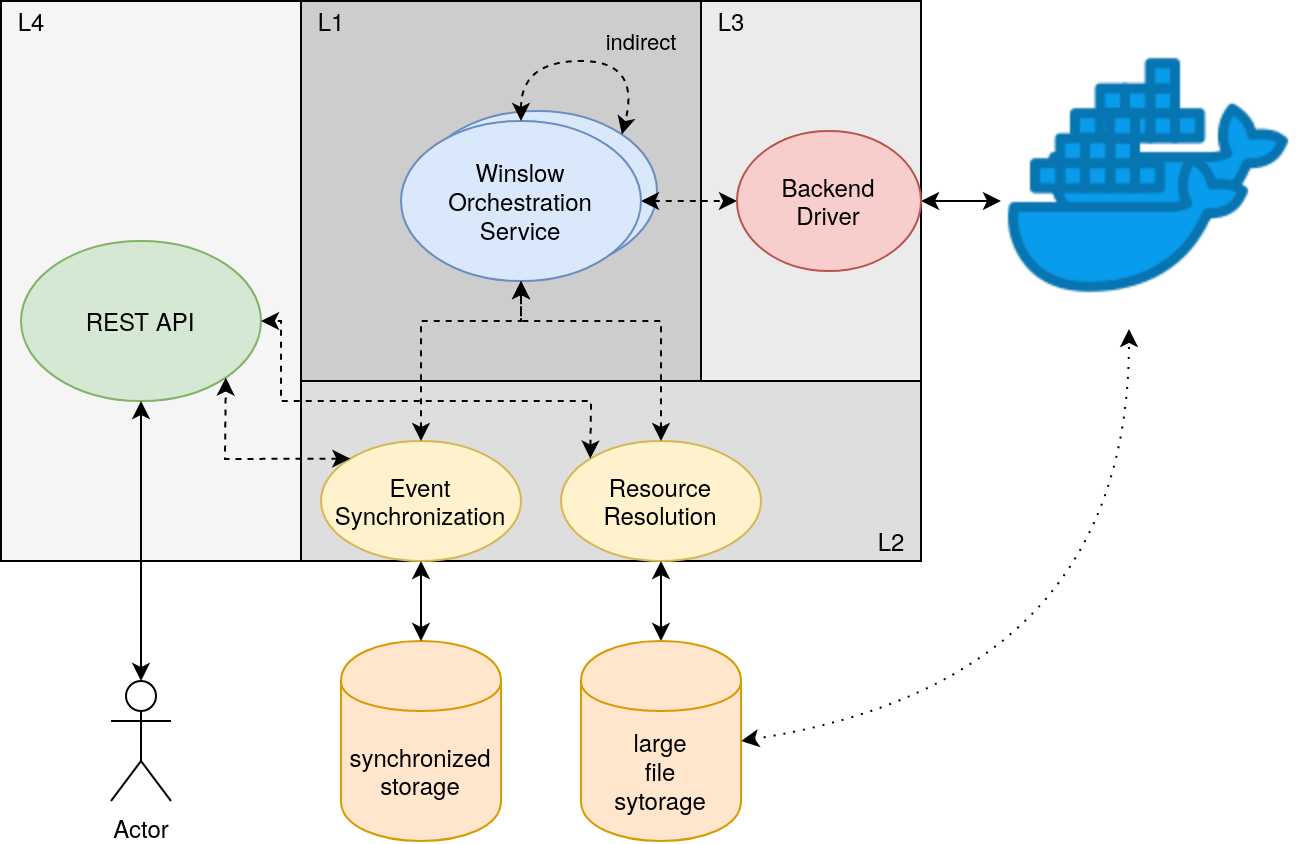
\includegraphics[width=0.95\textwidth]{architecture_detailed.png}
	\centering
	\caption{High level architecture overview of Winslow}
	\label{architecture:detailed}
\end{figure}

The meaning of the layers and their services will be explained in the following sub-sections.

\subsection{Layer 1: Orchestration Service}
\label{analysis:layer_1}

This layer is all about the fundamental business logic: when to schedule, start and abort which stage of what project a well as tracking the hardware utilization.
This level is also responsible to communicate these actions with all other Winslow instances, so that there is no duplicate or  missing stage execution or undetected node failure.

%The following requirements are therefore implemented here: \todo{.?}

\subsection{Layer 2: Events and Resources}
\label{analysis:layer_2}

The second layer is essential for the first layer to interact with and understand its environment.
It provides two important services: a synchronized communication channel and a large file storage.

The communication channel requires a storage to persist messages that are relevant for a duration of time.
It also needs to  support basic synchronization primitives to ensure consistency.
Winslow instances that have just been started need to see events that were issued before their start and which are still relevant to be able to replicate the system state correctly.

For executing stages, the system must be able to store large files.
The synchronized access can be ensured the event synchronization and thus the constraints to this storage is more relaxed than the one used to persist synchronization messages.
%An eventual consistent\todo{cite} storage could be used here. \todo{inter-stage synchronization? eventual-consistent might not be sufficient here?}


\subsection{Layer 3: Backend Driver}
\label{analysis:layer_3}


This layer is responsible to interface with Docker.
Once stage shall be executed, this driver is instructed to start a certain image with environment variables and the path to a prepared workspace.
By separating this task to its own layer it will be easier to change the Docker API for another implementation or to move away from the Docker platform at all if necessary.
A reason for this could be the change of needs, the appearance of a platform that is fulfilling the needs better or the disappearance of the currently used platform.
The latter sounds not that common at first, but the recent partial acquisition of Docker Inc by Mirantis\cite{docker:acquisition} proves that even very popular third party software is not going to be around for all eternity.
By moving the driver implementation into its own layer, but leaving the interface definition in layer 1, the driver implementation can be replaced easily without modifications to the inner layer.
It then also complies to the \enquote{Dependency Inversion Principle}\cite[65]{goll2018entwurfsprinzipien}.

While this driver is not supposed to access any storage itself, the stages need to read and write to the large file storage.
Docker does support mounting local directories or remote NFS shares as volumes into the container natively, access from within the executed stage can then also be guarded to limit read and write access to only the required working directories.

\subsection{Layer 4: Client Communication}

The final layer in this architecture is the client communication layer.
This service is not crucial for the actual execution and may be disabled on Winslow instances that shall not respond to a user requests.
A reason for this could be, that SSL certificates are bound to sub-domain which might point to specific Winslow instances and any unsecure access is not desired.
The REST API in this layer shall provide resources that can be accessed from the statically served Angular Web-Application\footnote{see \autoref{fundamental:angular}} or from future tools to upload or download files, to control stage execution and to monitor usage and logs.
%Removing or disabling this layer is not stopping the Winslow
